% 图 7.8 (a) 无磁场时的连续谱块（顶 E_⊥，x = E_⊥−E_l）(b) 分立朗道能级梯
\documentclass[tikz,border=5pt]{standalone}
\usetikzlibrary{arrows.meta}
\usepackage{amsmath}
\usepackage{bm}
\usepackage{fontspec}
\setmainfont{Times New Roman}
\begin{document}
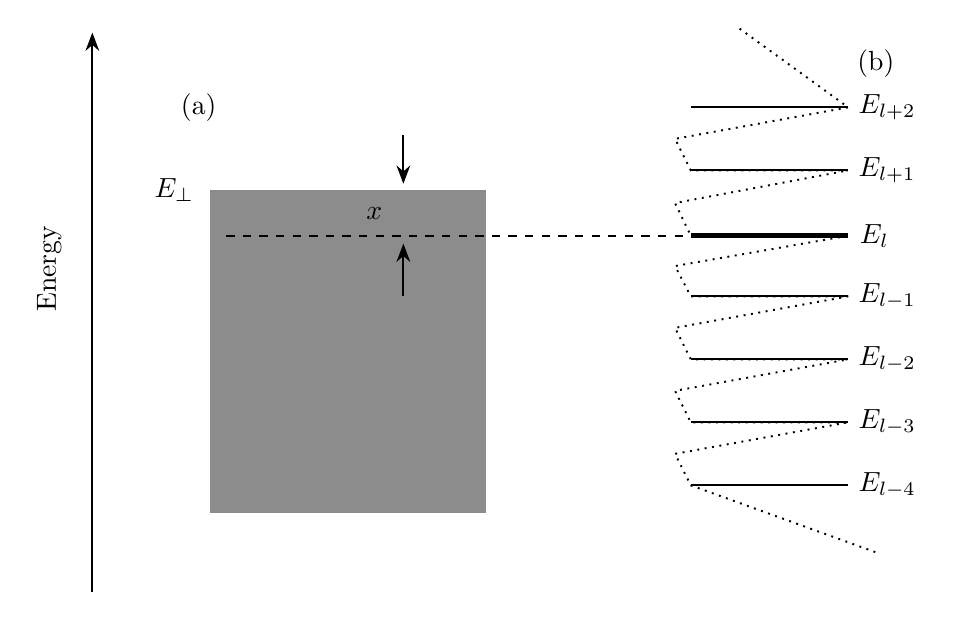
\begin{tikzpicture}[line width=0.8pt,>=Stealth]
% Energy 轴
\draw[->] (-0.6,0.2) -- (-0.6,7.3);
\node[rotate=90] at (-1.15,4.3) {Energy};
% ---------- (a) 连续谱块 ----------
\node at (0.75,6.35) {(a)};
\fill[black!45] (0.9,1.2) rectangle (4.4,5.3);
\node[left] at (0.82,5.3) {$E_\perp$};
% x 标记：块顶与点划线之间，两枚相向小箭头
\draw[dashed,line width=0.6pt] (1.1,4.72) -- (7.0,4.72);
\draw[->] (3.35,6.0) -- (3.35,5.38);
\draw[->] (3.35,3.95) -- (3.35,4.62);
\node at (2.98,5.0) {$x$};
% ---------- (b) 朗道能级梯 ----------
\node at (9.35,6.9) {(b)};
% 能级：E_l 加粗，其余细线
\draw[line width=0.8pt] (7.0,6.35) -- (9.0,6.35) node[right] {$E_{l+2}$};
\draw[line width=0.8pt] (7.0,5.55) -- (9.0,5.55) node[right] {$E_{l+1}$};
\draw[line width=1.7pt] (7.0,4.72) -- (9.0,4.72) node[right] {$E_l$};
\draw[line width=0.8pt] (7.0,3.95) -- (9.0,3.95) node[right] {$E_{l-1}$};
\draw[line width=0.8pt] (7.0,3.15) -- (9.0,3.15) node[right] {$E_{l-2}$};
\draw[line width=0.8pt] (7.0,2.35) -- (9.0,2.35) node[right] {$E_{l-3}$};
\draw[line width=0.8pt] (7.0,1.55) -- (9.0,1.55) node[right] {$E_{l-4}$};
% 相邻能级间点状锯齿折线（顶、底各延伸一段）
\draw[dotted,line width=0.7pt] (7.62,7.35) -- (9.0,6.35)
  -- (6.8,5.95) -- (7.0,5.55) -- (9.0,5.55)
  -- (6.8,5.135) -- (7.0,4.72) -- (9.0,4.72)
  -- (6.8,4.335) -- (7.0,3.95) -- (9.0,3.95)
  -- (6.8,3.55) -- (7.0,3.15) -- (9.0,3.15)
  -- (6.8,2.75) -- (7.0,2.35) -- (9.0,2.35)
  -- (6.8,1.95) -- (7.0,1.55) -- (9.35,0.7);
\end{tikzpicture}
\end{document}
